\documentclass{standalone}
\usepackage{tikz}
\usetikzlibrary{arrows,decorations.markings,calc,positioning}

% "Add arrows to a smooth tikz function"
% from http://tex.stackexchange.com/a/163695
\tikzset{
   set arrow inside/.code={\pgfqkeys{/tikz/arrow inside}{#1}},
   set arrow inside={end/.initial=>, opt/.initial=},
   /pgf/decoration/Mark/.style={
      mark/.expanded=at position #1 with
      {
         \noexpand\arrow[\pgfkeysvalueof{/tikz/arrow inside/opt}]{\pgfkeysvalueof{/tikz/arrow inside/end}}
      }
   },
   arrow inside/.style 2 args={
      set arrow inside={#1},
      postaction={
         decorate,decoration={
            markings,Mark/.list={#2}
         }
      }
   },
}

\begin{document}%
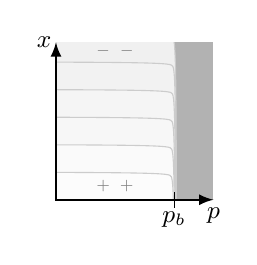
\begin{tikzpicture}[font=\small]

% contours
\begin{scope}
   \fill[black!30] (0,0) rectangle (2.0,2.0);
   \clip (0,0) rectangle (2.0,2.0);
   \foreach \s in {6,...,1}
   {
      %\begin{scope}[shift={($(0.35*\s,0.35*\s)$)}]
      \begin{scope}[shift={($(1.5+0.005*\s,0.35*\s)$)}]
      
         \coordinate (parama) at (-0.5, 0.0);
         \coordinate (paramb) at (-0.05, 0.0);
         \coordinate (paramc) at ( 0.0,-0.05);
         \coordinate (paramd) at ( 0.0,-0.5);
      
         \draw[black!20,fill=black!\s]
         (-5.0,0.0) .. controls (parama) and (paramb) .. 
         (-0.05, -0.05) .. controls (paramc) and (paramd) .. (0.0,-5.0)
          -- (-5.0,-5.0) -- cycle;
          
         %\node[circle,fill=blue,inner sep=0.1cm] at (parama) {};
         %\node[circle,fill=blue,inner sep=0.1cm] at (paramb) {};
         %\node[circle,fill=blue,inner sep=0.1cm] at (paramc) {};
         %\node[circle,fill=blue,inner sep=0.1cm] at (paramd) {};
         
      \end{scope}
   }
\end{scope}

\node[text=black!50] at (0.6,0.17) {\tiny $+$};
\node[text=black!50] at (0.9,0.17) {\tiny $+$};
\node[text=black!50] at (0.6,1.89) {\tiny $-$};
\node[text=black!50] at (0.9,1.89) {\tiny $-$};

%\draw[black!5] (-0.1,-0.1) rectangle (3.6,3.6);

%\draw[black!50] (-0.1,0.7) -- (3.5,0.7); % optimal path
%\node at (1.75,0.9) {\scriptsize Optimal Path};

% simple point
%\node[circle,fill=black,inner sep=0.07cm] at (1.5,3) {};
%\node[circle,fill=black,inner sep=0.05cm] (a1) at (1.0,2.7) {};
%\node[above right=-0.1cm of a1] {$A_1$};

%\node[circle,fill=black,inner sep=0.05cm] (a2) at (2.4,1.7) {};
%\node[above right=-0.1cm of a2] {$A_2$};

% anytime
%\draw[black,thick,->,
%   arrow inside={end=>,opt={black}}{0.25,0.5,0.75}]
%   (0.84,2.45)
%   .. controls (1.05,1.96) and (1.54,1.96) .. (1.96,1.75)
%   .. controls (2.38,1.54) and (2.67,0.84) .. (3.50,0.77);
%\node[circle,fill=black,inner sep=0.07cm] at (2.45,1.33) {};

% axes
\draw[thick,latex-latex] (2.0,0) -- (0,0) -- (0,2.0);

% labels
\node at (2.0,-0.2) {$p$};
\node at (-0.15,2.0) {$x$};

\draw[black] (1.5,-0.1) -- (1.5,0.1);
\node at (1.5,-0.25) {$p_b$};

%\node at (-0.2,0.75) {$x^*$};

%\node[anchor=east,inner sep=0pt] at (3.5,0.2) {\scriptsize Planning Effort $\rightarrow$};
%\node[rotate=90,anchor=east,inner sep=0pt] at (0.2,3.5) {\scriptsize Execution Effort $\rightarrow$};

\end{tikzpicture}%
\end{document}
